\documentclass[12pt]{extarticle}
\usepackage{hyperref}
\usepackage[margin=1in]{geometry}
% \usepackage{tabularx}
% \usepackage{xcolor-material}
% \usepackage{cancel}
% \usepackage{ulem}
\usepackage{graphicx}
\usepackage{listingsutf8}
\usepackage{color}
\usepackage[section]{placeins}

\lstdefinestyle{mystyle}{
    backgroundcolor=\color{backcolour},
    basicstyle=\scriptsize
}
 
\lstset{style=mystyle}

\definecolor{backcolour}{rgb}{0.95,0.95,0.92}

% \renewcommand\tabularxcolumn[1]{m{#1}}% for vertical centering text in X column

\begin{document}
\begin{titlepage}
\centering
{\LARGE\bfseries Tecnologie WEB}

\vspace{1cm}

{\Large Relazione Progetto}

\vspace{0.2cm}
{\large (a.a. 2019-2020)}

\vspace{2cm}

{\large Alexandru MOCANU}

\vspace{0.2cm}

{\small Matr. 813322}


\vspace{2cm}

% {\bfseries Submitted in fulfillment of the degree \ldots}

\vfill

{\itshape Università degli Studi di Torino - Dipartimento di Informatica}
\end{titlepage}

% Other content goes here...
\tableofcontents

\clearpage

\section{Presentazione del sito}
\subsection{Tematica del sito}
TWebShop è un sito di e-commerce che vende smartphone attraverso un catalogo sempre
aggiornato e in continua espansione.
\\
Vengono trattati i brand più famosi presenti sul mercato, come Apple, Samsung e Huawei.

\subsection{Sezioni principali}
\subsubsection{Login/Registrazione}
L'utente, per poter usufruire dei vari servizi del sito, ha bisogno di
accedere attraverso le sue credenziali. Se l'utente in questione non le possiede può registrarsi
fornendo le sue informazioni. Dopo aver effettuato il login sarà caricata l'homepage del sito, e
sarà possibile accedere a tutte le varie pagine del sito.

\subsubsection{Homepage}
Effettuato il login, l'utente sarà indirizzato alla seguente pagina. Qui l'utente ha la
possibilità di:
\begin{itemize}
    \item  visualizzare il catalogo del sito;
    \item selezionare un prodotto per ottenere nuove informazioni, come ad esempio caratteristiche e recensioni;
    \item effettuare una ricerca;
    \item aggiungere uno o più prodotti nel Carrello e nella Wishlist
\end{itemize}

\subsubsection{Prodotto}
In questa pagina l'utente può visualizzare le varie caratteristiche del prodotto (prezzo,
memoria, sistema operativo ecc.) e le recensioni, se presenti. Tramite questa pagina l'utente
può aggiungere il prodotto selezionato nel suo Carrello o nella sua Wishlist.

\subsubsection{Carrello}
In questa pagina sono presenti i vari smartphone aggiunti dall'utente. Da qui è
possibile completare l'acquisto o trasferire il prodotto nella Wishlist

\subsubsection{Wishlist}
In questa pagina sono presenti i vari smartphone aggiunti dall'utente. Questa pagina
ha lo scopo di salvare i prodotti che colpiscono l'utente. Da qui è possibile trasferire il prodotto
nel Carrello.
\subsubsection{Buy}
Qui vengono aggiunte tutte le informazioni per la spedizione del prodotto. Oltre a questo
vengono mostrate le informazioni relative al prodotto e al suo acquisto (nome del prodotto,
spese di spedizione, eventuali sconti ecc.)

\subsubsection{Ordini}
Qui vengono mostrati tutti gli ordini completati e le informazioni relative.
 Inoltre tramite questa pagina è possibile rilasciare recensioni del prodotto.

\subsubsection{Game}
in questa pagina è possibile giocare per ottenere sconti sul prossimo acquisto. 


\subsection{Schema di navigazione di base}
\subsubsection{Header}
Il sito possiede un header dove è possibile svolgere diverse operazioni. Tramite l'header l'utente,
dopo aver effettuato il login, può accedere alle diverse pagine del sito, fatta eccezione per le
pagine product e buy tramite le varie icone che rappresentano le diverse pagine. Oltre a queste
icone ne è presente un'altra che ha lo scopo di disconnettere l'utente quando esso lo vorrà. Se
l'utente non ha ancora effettuato l'accesso questa icona non sarà mostrata. Se l'utente non ha
effettuato l'accesso e seleziona qualsiasi delle varie icone, il sito indirizzerà l'utente alla pagina di
login del sito.

% \includegraphics[width=\textwidth]{er1.png}

\subsubsection{Login/Registrazione}
Come già accennato precedentemente, qui l'utente può effettuare il login o la registrazione.
Per quanto riguarda il login l'utente dovrà inserire il suo username e la password. Se queste
saranno valide l'utente sarà indirizzato alla homepage del sito. In caso contrario verrà ricaricata la
pagina con l'aggiunta della motivazione del mancato accesso.
Per la registrazione, invece, l'utente dovrà inserire diverse informazioni (username, nome,
cognome, email e password). Se la registrazione avverrà con successo verrà ricaricata la pagina;
qui l'utente potrà effettuare il login. Se la registrazione fallirà, invece, verrà ricaricata la pagina con
l'aggiunta della motivazione della registrazione fallita.

\subsubsection{Home}
In questa pagina l'utente può svolgere diversi compiti.
È presente il catalogo del sito e qui l'utente può selezionare un prodotto per ottenere ulteriori
informazioni sullo smartphone selezionato.
Sono presenti tre banner: il primo per il Carrello, il secondo per il Gioco e il terzo per la Wishlist.
L'utente potrà trascinare i prodotti nel banner del Carrello o della Wishlist per aggiungerli in uno
dei due. Questo avviene tramite la funzione drag and drop. Se saranno già presenti, i prodotti
trascinati e rilasciati non saranno aggiunti nuovamente e ciò verrà notificato all'utente.
È presente una barra di ricerca che permette all'utente di ricercare un prodotto. Questa barra di
ricerca è stata creata con l'ausilio di Autocompleter.

\subsubsection{Product}
Qui vengono mostrate tutte le informazioni del prodotto in questione.
Tramite dei bottoni l'utente può aggiungere il prodotto nel Carrello e nella Wishlist. Se il prodotto è
già presente nel Carrello o nella Wishlist, il prodotto non sarà aggiunto e ciò verrà notificato
all'utente. Se il prodotto non è più disponibile, l'utente potrà solamente aggiungerlo nella Lista dei
Desideri. Oltre a ciò sono mostrate, se presenti, tutte le recensioni dello smartphone scritte dagli
utenti del sito. 

\subsubsection{Cart}
In questa pagina vengono mostrati tutti gli smartphone aggiunti nel Carrello. Qui l'utente potrà
spostare il prodotto nella Wishlist o eliminarlo tramite dei bottoni. Oltre a questo l'utente può
selezionare la tipologia di spedizione e acquistare il prodotto tramite un terzo bottone. Se il
prodotto non è più disponibile, l'utente non potrà acquistarlo

\subsubsection{Wishlist}
In modo simile alla pagina del Carrello, in questa pagina vengono mostrati tutti gli smartphone
aggiunti nella Wishlist. Qui l'utente potrà spostare il prodotto nel Carrello o eliminarlo tramite dei
bottoni.

\subsubsection{Orders}
In questa pagina vengono mostrati tutti gli smartphone acquistati dall'utente. Tramite questa
pagina l'utente potrà tornare alla pagina dello smartphone cliccando sulla sua immagine. Qui sarà
possibile scrivere le recensioni tramite la compilazione di un form. L'utente potrà recensire il
prodotto solamente una volta.

\subsubsection{Buy}
È possibile arrivare in questa pagina solamente tramite la pagina Cart, dopo aver selezionato un
determinato prodotto. Qui bisognerà aggiungere tutte le informazioni necessarie per la spedizione
del prodotto. Questo avverrà tramite la compilazione di un form. Cliccando su un bottone
dedicato si potrà confermare l'acquisto. Quando sarà completato verrà mostrato la conferma (o
no) dell'acquisto.

\subsubsection{Game}
In questa pagina è possibile giocare per ottenere uno sconto. Lo scopo del gioco è quello di
indovinare 4 smartphone su 5 entro un certo tempo. Saranno mostrati 5 immagini di smartphone,
ottenuti dal catalogo del sito, in formato puzzle. In caso di vittoria l'utente otterrà uno sconto da 
utilizzare per il suo prossimo acquisto (lo sconto verrà applicato automaticamente poco prima
della conferma dell'acquisto).


\subsubsection{Footer}
In ogni pagina, tranne per la pagina di Login, è presente un footer. Qui sono presenti i vari nomi
delle sezioni del sito. Cliccando su una di esse l'utente verrà indirizzato alla pagina selezionata

\subsection{Mockup}
\FloatBarrier
\begin{figure}
    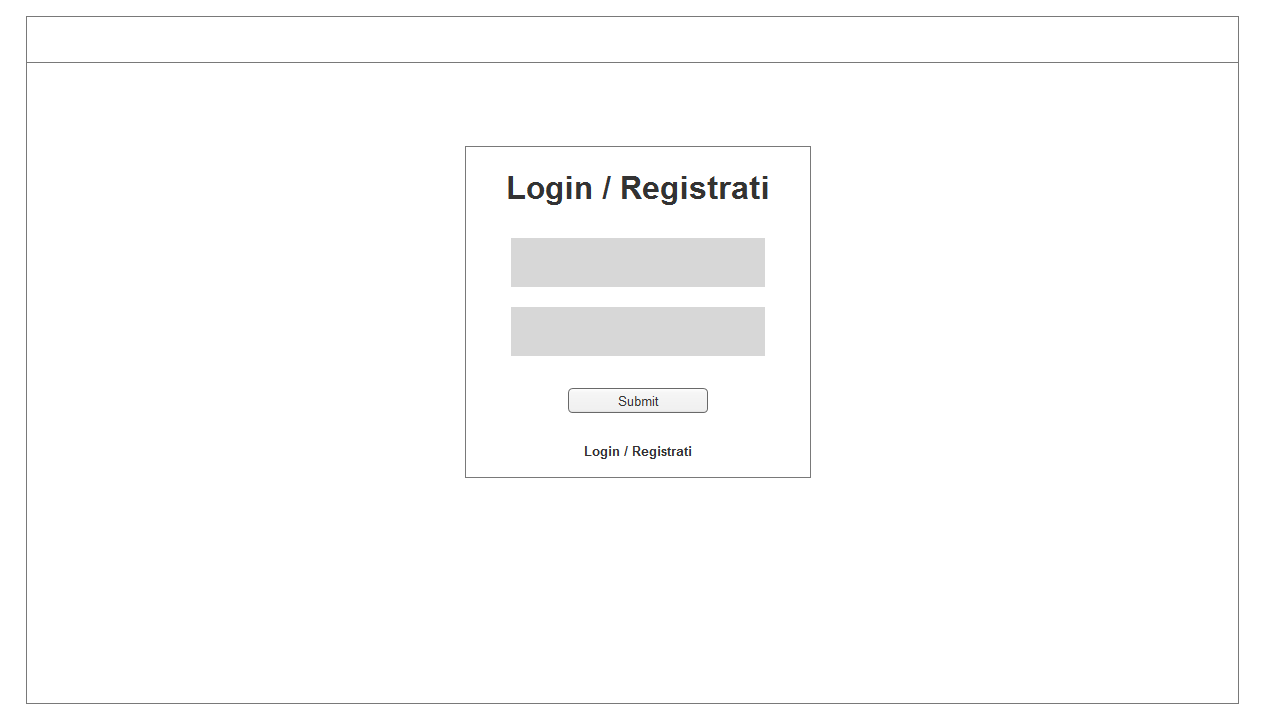
\includegraphics[width=\linewidth]{mocanu/mockup/Index.png}
    \caption{index.php}
    \label{fig:index.php}
\end{figure}
\begin{figure}
    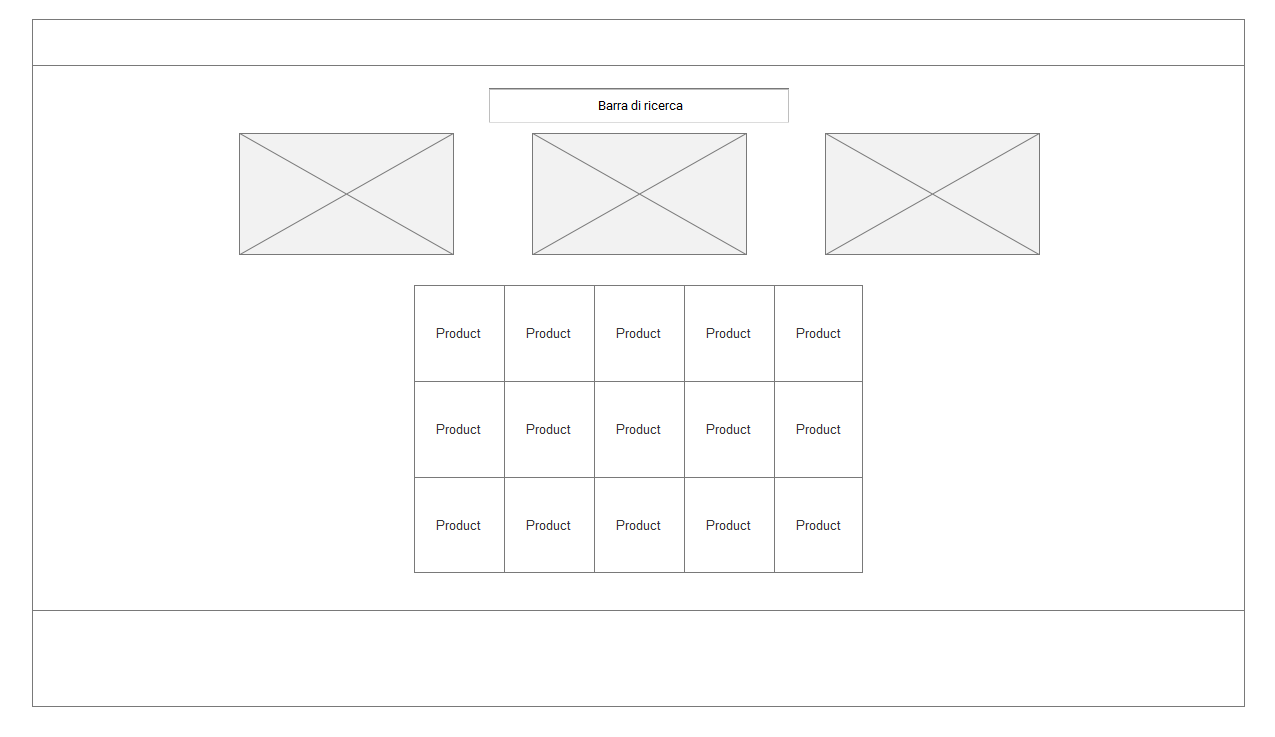
\includegraphics[width=\linewidth]{mocanu/mockup/Home.png}
    \caption{home.php}
    \label{fig:home.php}
\end{figure}
\begin{figure}
    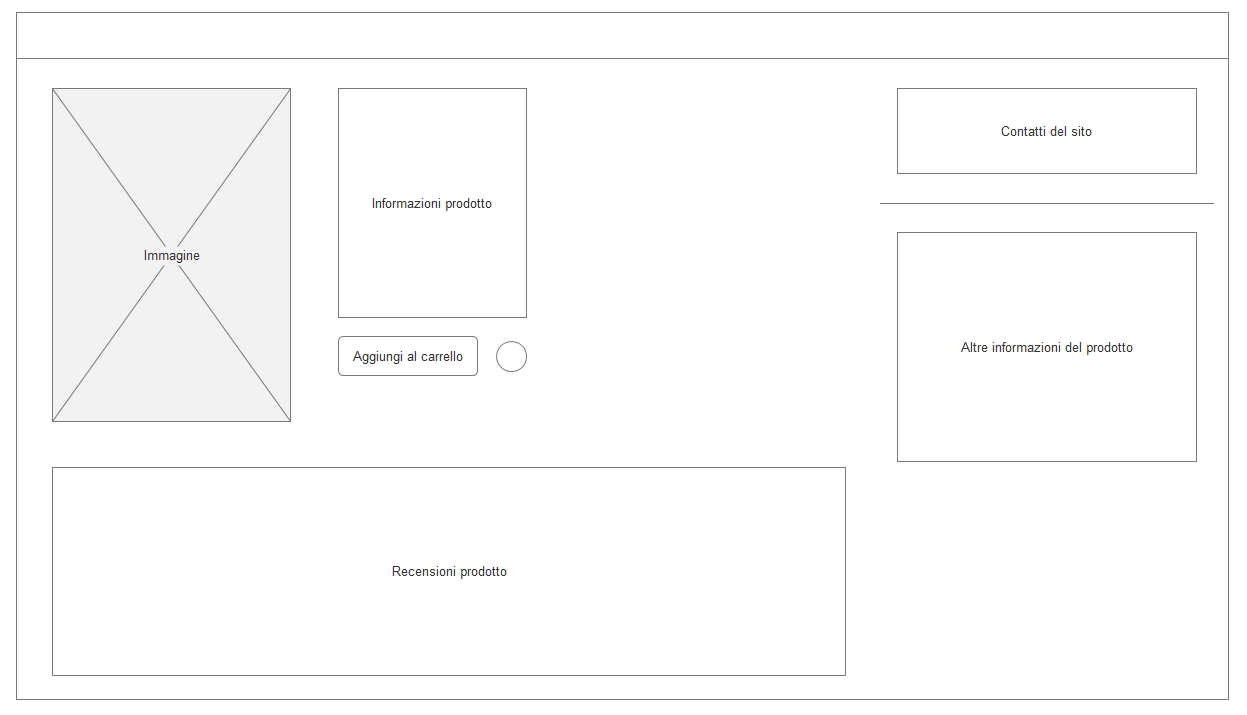
\includegraphics[width=\linewidth]{mocanu/mockup/Product.png}
    \caption{product.php}
    \label{fig:product.php}
\end{figure}
\begin{figure}
    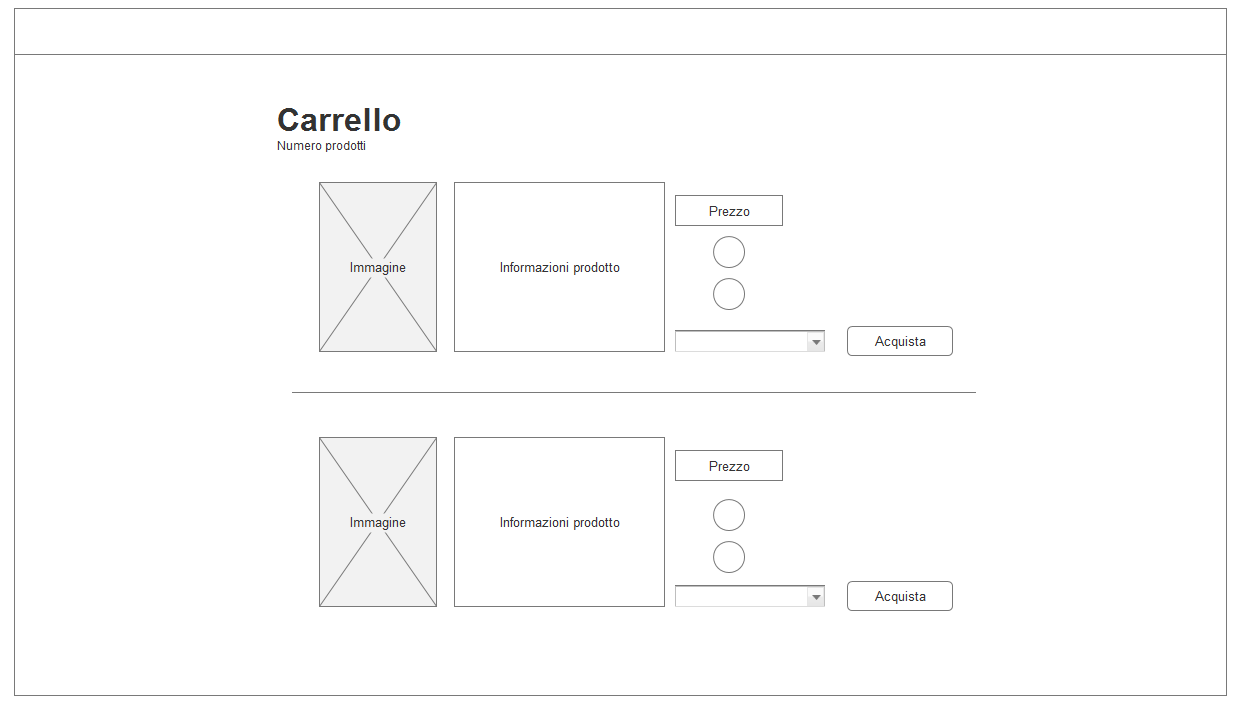
\includegraphics[width=\linewidth]{mocanu/mockup/Carrello.png}
    \caption{cart.php}
    \label{fig:cart.php}
\end{figure}
\begin{figure}
    \includegraphics[width=\linewidth]{mocanu/mockup/wishlist.png}
    \caption{wish.php}
    \label{fig:wish.php}
\end{figure}
\begin{figure}
    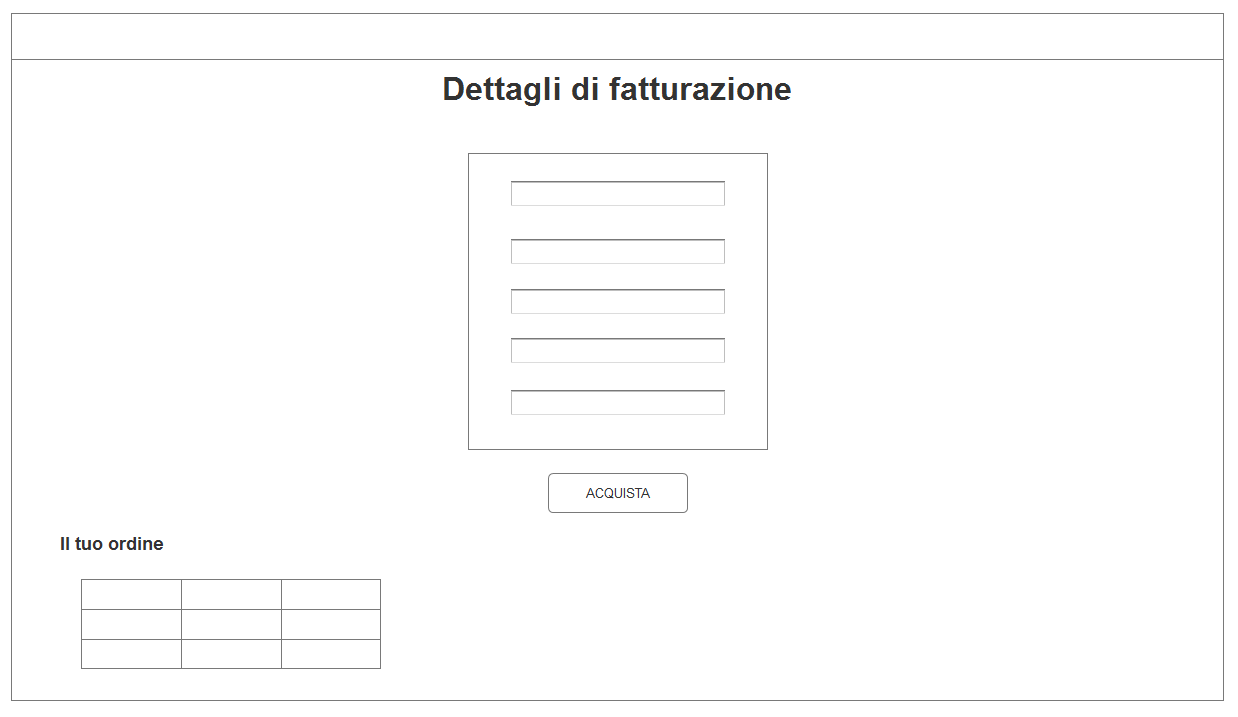
\includegraphics[width=\linewidth]{mocanu/mockup/Buy.png}
    \caption{buy.php}
    \label{fig:buy.php}
\end{figure}
\begin{figure}
    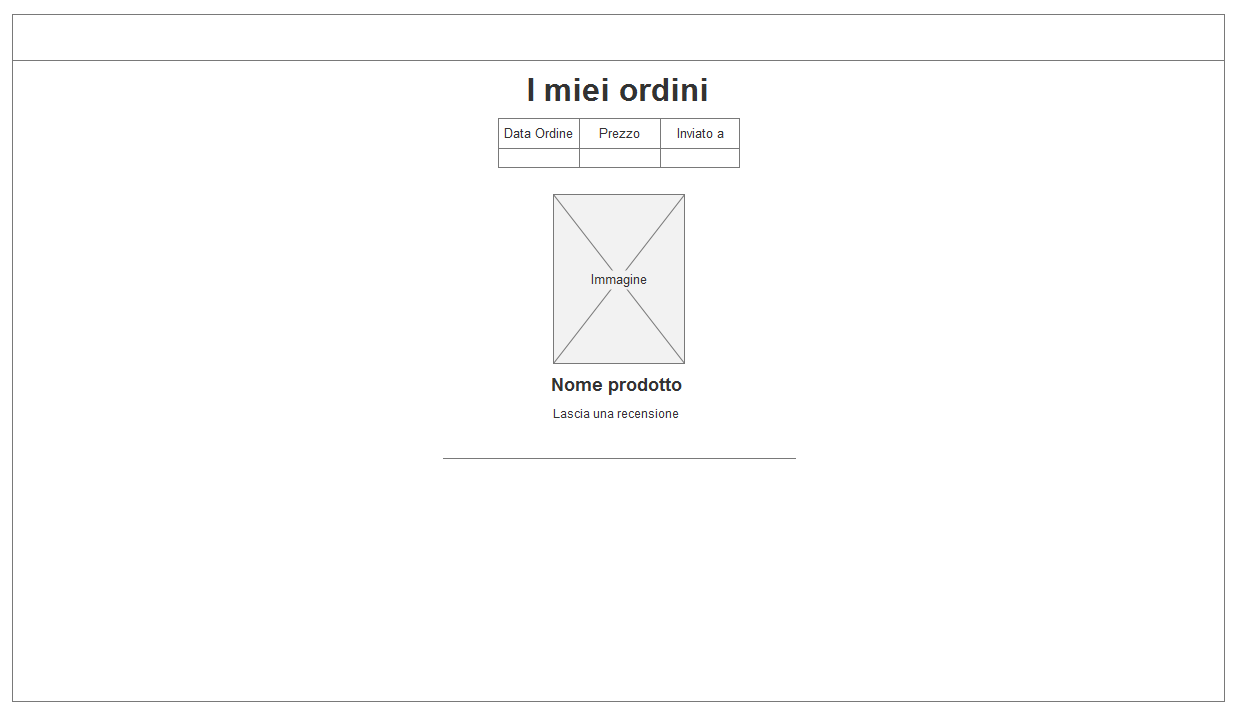
\includegraphics[width=\linewidth]{mocanu/mockup/Ordini.png}
    \caption{orders.php}
    \label{fig:orders.php}
\end{figure}
\begin{figure}
    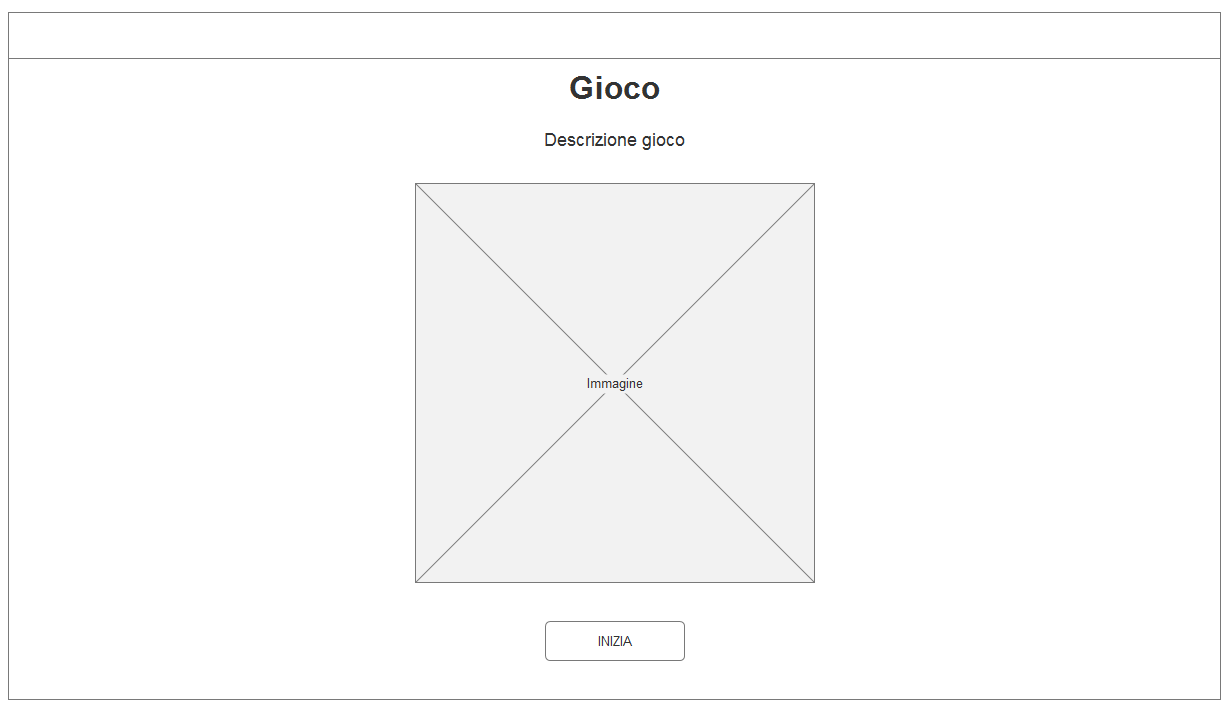
\includegraphics[width=\linewidth]{mocanu/mockup/Gioco.png}
    \caption{game.php}
    \label{fig:game.php}
\end{figure}



\section{Funzionalità del sito}

\subsection{Login/Registrazione}
Il Login e la Registrazione sono stati implementati nella pagina \textit{index.php}. Verrà mostrato
solamente il form del Login. Da qui si può passare al form della registrazione tramite il click su un
link (in seguito viene nascosto il form del Login e mostrato il form della Registrazione).
Per entrambi i form, cliccando sul tasto "Accedi/Registrati" viene chiamata una funzione Ajax
dal client al server tramite \textit{loginregister.js}. La richiesta è di tipo POST e i dati mandati
saranno composti da diverse informazioni (username e password per il Login; username, nome,
cognome ecc. per la Registrazione). In caso di Login il server, dopo aver ottenuto i dati, verifica la
corrispondenza delle informazioni con il database. Se l'operazione ha successo il server
consegna l'esito, in JSON, dell'operazione. Il client, dopo aver ottenuto l'esito, indirizza l'utente
nella homepage in caso di successo o nella stessa pagina in caso di fallimento. Per quanto
riguarda la Registrazione, invece, il server verifica che username e email non siano già presenti nel
database. Anche qui se l'operazione ha successo il server consegna l'esito, sempre in JSON
dell'operazione. Qualsiasi sia l'esito l'utente sarà indirizzato nuovamente nella stessa pagina e
visualizzerà l'esito della Registrazione.

\subsection{Logout}
Se l'utente ha effettuato l'accesso, esso può disconnettersi tramite il click sull'immagine presente
nell'header. Cliccando l'icona avviene una chiamata Ajax dal client al server tramite \textit{logout.js}.
La richiesta è di tipo GET e non vengono mandati dati dal client al server. Quest'ultimo può
effettuare la disconnessione tramite la distruzione (\textit{session\_unset()} e \textit{session\_destroy()}) della
sessione generata dall'utente. Quest'ultimo quindi viene indirizzato alla pagina di Login

\subsection{Contenuto generato dall'utente}
Nella pagina Carrello vengono mostrati i prodotti aggiunti dall'utente; questo è necessario per
completare un acquisto. L'aggiunta dei prodotti nel Carrello avviene tramite \textit{addToCart.js} e
\textit{addToCart.php} grazie a Ajax.
Anche nella pagina Wishlist avviene ciò. Questa pagina è utile per "salvare" i prodotti interessanti.
L'aggiunta dei prodotti nella Wishlist avviene tramite \textit{addToWish.js} e \textit{addToWish.php} grazie a
Ajax.
L'utente può aggiungere prodotti nel Carrello o nella Wishlist in tre modi: dalla home, dalla pagina
del prodotto o dal Carrello/Wishlist.
L'utente oltre a questo può scrivere recensioni per i prodotti acquistati. Le recensioni possono
essere scritte dalla pagina degli Ordini. Le recensioni scritte verranno mostrate nella pagina del
prodotto in questione. Questo avviene tramite \textit{order.js} e \textit{addReview.php} (anche qui si sfrutta
Ajax).



\section{Caratteristiche}
\subsection{Usabilità}
È stato curato l'aspetto e facilità d'uso con lo scopo di creare un look\&feel ottimale. Sono stati
utilizzati colori e sfondi semplici, con l'obiettivo di avere uno stile coerente in tutte le pagine. È
stata data molta attenzione all'esperienza utente: per questa ragione il sito è stato mostrato a
diverse persone in modo da capire quali fossero le funzioni meno intuitive.

\subsection{Sessioni}
Le funzioni session\_start(), session\_regenerate\_id(), session\_unset(), e
session\_destroy() sono state utilizzate nell'ordine adeguato. Queste funzioni si trovano nei
seguenti file: \textit{common.php, loginuser.php} e logout.php.
Le variabili \$\_SESSION sono le seguenti: \$\_SESSION['user'] e \$\_SESSION['product'].

\subsection{Interrogazioni del database}
Le query del database hanno una rilevanza fondamentale. Vengono utilizzate per la maggior parte
delle funzioni presenti nel sito. Per le interrogazioni è stato implementato PDO. Le diverse query
utilizzate si trovano in tutte i file presenti nella cartella Model

\subsection{Validazione dati input}
La validazione dei dati avviene in diversi casi:
\begin{itemize}
    \item login: si verifica che i dati sia quelli presenti nel database, in modo da confermare l'identità dell'utente; 
    \item registrazione: si verifica che i dati (username e mail) non siano già presenti nel database;
    \item carrello: si verifica che il prodotto in questione non sia già presente nel Carrello;
    \item wishlist: si verifica che il prodotto in questione non sia già presente nella Wishlist;
    \item nuova recensione: si verifica che l'utente non abbia già scritto una recensione per un determinato prodotto, in modo da non permettere una seconda recensione.
\end{itemize}

\subsection{Sicurezza}
Sono stati bloccati tentativi malevoli riguardo ad attacchi via URL o via Information leakage.
Per quanto riguarda le query in PHP viene applicata la funzione quote(). Per le password degli
utenti si utilizza la funzione di password\_hash().

\subsection{Presentazione}
Come già anticipato, si è puntato alla realizzazione di un sito semplice ma intuitivo, in modo da
avere un layout chiaro e leggibile. Lo stile di ogni pagina è coerente con il resto.


\section{Front-end}
\subsection{Separazione presentazione/contenuto/comportamento}
È stato utilizzato uno stile unobtrusive in modo da rendere il codice generale pulito e chiaro.
Questo è stato realizzato grazie all'utilizzo di jQuery.
\\
Il contenuto di ogni pagina è realizzato tramite file \textit{.js}, che si occupano di popolare il DOM con le
informazioni richieste (esempio: nel Carrello saranno presenti tutti i prodotti aggiunti dall'utente
connesso).
\\
La connessione tra client e server avviene mediante l'ausilio delle chiamate Ajax.
Come già anticipato, le pagine che l’utente può visualizzare corrispondono alle sezioni citate
precedentemente.
\\
Gli unici file .html sono quelli riguardanti l'inizializzazione e terminazione di ogni pagina presente
nel sito, ossia top.html e bottom.html.

\subsection{Soluzioni cross-platform}
Il sito è stato testato su Google Chrome (Versione 79) e Firefox (versione 72.0)

\subsection{Organizzazione file e cartelle di progetto}
\begin{itemize}
    \item All'interno della cartella controller sono presenti tutti i file \textit{.js}
    \item All'interno della cartella model sono presenti i file \textit{.php} che
    hanno il compito si svolgere le varie query e di ritornare i risultati.
    \item All'interno della cartella view sono presenti i file .html e \textit{.php} che
    si occupano della "vista" del sito. Oltre a questi file sono presenti
    quelli .css
\end{itemize}

\section{Back-end e comunicazione Front/Back-end}
\subsection{Architettura generale classi/funzioni php}
Le varie funzioni php sono suddivise in base al loro compito.

\subsubsection*{funzioni generali}
\begin{itemize}
    \item \textit{common.php}: verifica che l'utente sia connesso e ha la maggior parte delle funzioni in esso
    \item \textit{dbconnect.php}: connessione al database
    \item funzioni generiche per ottenere informazioni dal db
\end{itemize}

\subsubsection*{users}
\begin{itemize}
    \item \textit{loginuser.php}: login dell'utente
    \item \textit{registeruser.php}: registrazione dell'utente
    \item \textit{logoutuser.php}: logout dell'utente
\end{itemize}

\subsubsection*{orders}
\begin{itemize}
    \item \textit{addReview.php}: inserimento di una nuova recensione
    \item \textit{checkReviews.php}: viene verificato che l'utente non stia cercando di inserire una seconda
    recensione sullo stesso prodotto
    \item \textit{getProductOrder.php}: informazioni dei prodotti acquistati da un utente
    \item \textit{infoOrders.php}: ordini di un dato utente
\end{itemize}

\subsubsection*{product}
\begin{itemize}
    \item \textit{addToCart.php / addToWish.php}: inserimento di un prodotto nel Carrello o nella Wishlist
    \item \textit{addToCartFromWish.php}: inserimento di un prodotto nel Carrello dalla Wishlist
    \item \textit{addToWishFromCart.php}: inserimento di un prodotto nella Wishlist dal Carrello
    \item \textit{removeFromCart.php}: rimozione di un prodotto dal Carrello
    \item \textit{removeFromWish.php}: rimozione di un prodotto dalla
    \item \textit{getCart.php}: prodotti presenti nel Carrello
    \item \textit{getWish.php}: prodotti presenti nella Wishlist
    \item \textit{getProducts.php}: prodotti presenti nell'intero database
    \item \textit{infoProduct.php}: informazioni relative a un dato prodotto
    \item \textit{productReviews.php}: recensioni di un prodotto
\end{itemize}

\subsubsection*{home}
\begin{itemize}
    \item \textit{getProductsHome.php}: prodotti da mostrare nella home
    \item \textit{cartviadrop.php}: inserimento di un prodotto nel Carrello (tramite Drag \& Drop)
    \item \textit{wishviadrop.php}: inserimento di un prodotto nella Wishlist (tramite Drag \& Drop)
\end{itemize}

\subsubsection*{buy}
\begin{itemize}
    \item \textit{newOrder.php}: creazione di un nuovo ordine per un dato utente
\end{itemize}

\subsubsection*{game}
\begin{itemize}
    \item  \textit{discount.php}: funzione con lo scopo di aggiungere uno sconto a un dato utente
\end{itemize}

\FloatBarrier
\subsection{Schema del Database}
\begin{lstlisting}[language=SQL]
    TABLE user
        id INT, PRIMARY KEY, NOT NULL, AUTO_INCREMENT
        username VARCHAR, NOT NULL
        password VARCHAR, NOT NULL
        name VARCHAR, NOT NULL
        surname VARCHAR, NOT NULL
        mail VARCHAR, NOT NULL
        discount INT, NOT NULL
    
    TABLE product
        id INT, PRIMARY KEY, NOT NULL, AUTO_INCREMENT
        name VARCHAR, NOT NULL
        quantity INT, NOT NULL
        brand VARCHAR, NOT NULL
        price FLOAT, NOT NULL
        color VARCHAR, NOT NULL
        os VARCHAR, NOT NULL
        chipset VARCHAR, NOT NULL
        memory VARCHAR, NOT NULL
        ram VARCHAR, NOT NULL
        display VARCHAR, NOT NULL
        resolution VARCHAR, NOT NULL
        battery VARCHAR, NOT NULL
        primarycamera VARCHAR, NOT NULL
        secondarycamera VARCHAR, NOT NULL
        dimension VARCHAR, NOT NULL
        weigth VARCHAR, NOT NULL
        wlan VARCHAR, NOT NULL
        gps VARCHAR, NOT NULL
    
    TABLE cart
        id_user FLOAT, FOREIGN KEY, NOT NULL
        id_product FLOAT, FOREIGN KEY, NOT NULL
    
    TABLE wish
        id_user FLOAT, FOREIGN KEY, NOT NULL
        id_product FLOAT, FOREIGN KEY, NOT NULL
    
    TABLE ordine
        id INT, PRIMARY KEY, NOT NULL, AUTO_INCREMENT
        id_user FLOAT, FOREIGN KEY, NOT NULL
        id_product FLOAT, FOREIGN KEY, NOT NULL
        cost FLOAT, NOT NULL
        name VARCHAR, NOT NULL
        surname VARCHAR, NOT NULL
        address VARCHAR, NOT NULL
        city VARCHAR, NOT NULL
        cap INT, NOT NULL
        data VARCHAR, NOT NULL
    
    TABLE review
        id INT, PRIMARY KEY, NOT NULL, AUTO_INCREMENT
        id_user FLOAT, FOREIGN KEY, NOT NULL
        id_product FLOAT, FOREIGN KEY, NOT NUL
        title VARCHAR, NOT NULL
        description VARCHAR, NOT NULL
        data VARCHAR, NOT NULL
\end{lstlisting}

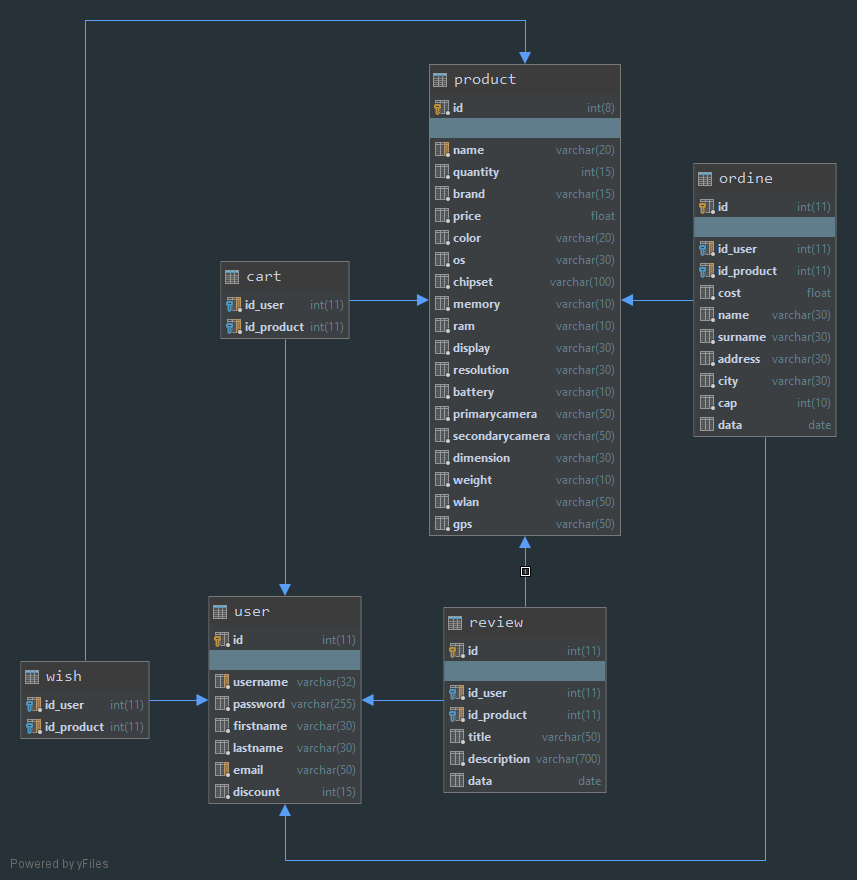
\includegraphics[width=\linewidth]{diagram.png}

\subsection{Gestione condizioni di errore}
Le condizioni di errore che possono presentarsi, quando l'utente immette input non corretti, sono
gestiti tramite Ajax via dati JSON. Sulla pagina del sito verrà mostrato un messaggio che
spiegherà il motivo dell'errore, in modo che l'utente possa capire la causa del problema.

\subsection{Funzioni di callback lato JavaScript/Ajax}

\subsubsection*{users}
\begin{itemize}
    \item \textit{loginregister.js}: sono presenti due chiamate Ajax, una per il login e una per la registrazione.
    Per quanto riguarda la registrazione, se la funzione ha successo viene mostrato l'esito
    tramite dati JSON.
    \item \textit{logout.js}: logout da parte dell'utente. Se la funzione ha successo l'utente viene reindirizzato
    alla pagina iniziale. Il valore di ritorno della chiamata è l'url della pagina iniziale.
\end{itemize}

\subsubsection*{product}
\begin{itemize}
    \item \textit{product.js}, \textit{cart.js} e \textit{wish.js}: sono presenti varie chiamate Ajax che hanno lo scopo di
ottenere informazioni fondamentali per il popolamento del DOM delle rispettive pagine
    \item \textit{addToCart.js}: come si evince dal titolo, la funzione ha il compito di inserire un prodotto nel
Carrello. Se la funzione ha successo viene mostrato all'utente l'esito dell'operazione tramite
dati JSON
    \item \textit{addToWish.js}: la funzione ha il compito di inserire un prodotto nella Wishlist. Se la funzione
ha successo viene mostrato all'utente l'esito dell'operazione tramite dati JSON
\end{itemize}

\subsubsection*{cart/wish}
\begin{itemize}
    \item \textit{cart.js} / \textit{wish.js}: sono presenti varie chiamate Ajax che hanno lo scopo di ottenere
    informazioni fondamentali per il popolamento del DOM della pagina.
\end{itemize}

\subsubsection*{home}
\begin{itemize}
    \item \textit{home.js}: sono presenti varie chiamate Ajax che hanno lo scopo di ottenere informazioni
    fondamentali per il popolamento del DOM della pagina. È presente la funzione di autocompletamento per la ricerca dei prodotti.
\end{itemize}

\subsubsection*{buy}
\begin{itemize}
    \item \textit{buy.js}: sono presenti varie chiamate Ajax che hanno lo scopo di ottenere informazioni
    fondamentali per il popolamento del DOM della pagina ((informazioni del prodotto, eventuali
    sconti dell'utente ecc.).
\end{itemize}

\subsubsection*{orders}
\begin{itemize}
    \item \textit{order.js}: sono presenti varie chiamate Ajax che hanno lo scopo di ottenere informazioni
    fondamentali per il popolamento del DOM della pagina (informazioni dei prodotti acquistati,
    informazioni sull'indirizzo degli ordini fatti ecc.).
\end{itemize}

\end{document}